
\documentclass[twocolumn,12pt]{article} % default is 10 pt
\usepackage{graphicx} % needed for including graphics e.g. EPS, PS

\long\def\comment#1{}

% uncomment if don't want page numbers
% \pagestyle{empty}

%set dimensions of columns, gap between columns, and paragraph indent 
\setlength{\textheight}{8.75in}
\setlength{\columnsep}{0.375in}
\setlength{\textwidth}{6.8in}
\setlength{\topmargin}{0in}
\setlength{\headheight}{0.0in}
\setlength{\headsep}{0.0in}
\setlength{\oddsidemargin}{-.19in}
\setlength{\parindent}{0pt}
\setlength{\parskip}{0.12in}
\makeatletter
\def\@normalsize{\@setsize\normalsize{10pt}\xpt\@xpt
\abovedisplayskip 10pt plus2pt minus5pt\belowdisplayskip 
\abovedisplayskip \abovedisplayshortskip \z@ 
plus3pt\belowdisplayshortskip 6pt plus3pt 
minus3pt\let\@listi\@listI}

%need an 11 pt font size for subsection and abstract headings 
\def\subsize{\@setsize\subsize{12pt}\xipt\@xipt}
%make section titles bold and 12 point, 2 blank lines before, 1 after
\def\section{\@startsection {section}{1}{\z@}{1.0ex plus
1ex minus .2ex}{.2ex plus .2ex}{\large\bf}}
%make subsection titles bold and 11 point, 1 blank line before, 1 after
\def\subsection{\@startsection 
   {subsection}{2}{\z@}{.2ex plus 1ex} {.2ex plus .2ex}{\subsize\bf}}
\makeatother

\begin{document}

% don't want date printed
\date{}

% >>>>>>>>>>>>>>>>>>>>>>>  Put your title here <<<<<<<<<<<<<<<<<<<<<<<<
% make title bold and 14 pt font (Latex default is non-bold, 16pt) 
\title{\Large {\bf System Design Project - Individual Report 4 }}

% >>>>>>>>>>>>>>>>>>>>>>> Author's Name, Thanks or Affliation <<<<<<<<
\author{Biser Hong - s0840625 - Group 12}
\maketitle
\thispagestyle{empty}


% >>>>>>>>>>>>>>>>>>>>>> START OF YOUR PAPER <<<<<<<<<<<<<<<<<<<<<<<<<<<<<<
% Typically paper starts of with an Introduction header.  Replace text in
% the french braces if you see fit.  I also typically name the label the
% same as the section

\section{Introduction}
\label{Introduction}

This report documents the major changes and improvements made since Milestone 3, and the updates on previously set goals. These include restructuring the code base, implementing a generalized collision detection algorithm, adding additional drawing functionality, and extending the prediction capabilities started just before Milestone 3.

\section{Simulator updates}
\label{Simulator updates}

\subsection{Collision detector}
\label{Collision detector}

Having had trouble managing all collisions by passing objects around to all other objects, I designed a central collision detection mechanism. Objects that need support for collisions are registered with a collision detector, and all relevant parties are notified in the case of a collision. The collision detector requests each object to send their shape on every update cycle. For every corner of that shape is tested to establish whether it falls within any of the other registered objects' shape. If this is the case, a collision packet, which includes the type of collision and the side of the shape that is closest to the other shape's corner, is constructed and sent to each object participating in the collision. 

% >>>>>>>>>>>>>>>>>>>>>>>>>>> Example of including a figure <<<<<<<<<<<<<<<<<<<<<<

\subsection{Improved drawing}
\label{Improved drawing}

As the strategy was becoming more and more complex, efficient debugging methods needed to be employed, especially in the case of finding logical errors in the code, which were usually harder to detect. Since any strategy involved fine tuning and certain thresholds were inevitable, a simple but useful transparent oval was drawn whenever there is a need to visualize, for example, the area around a point to which the robot needed to move. This ensured calculations were always correct and strategy is proceeding as it should (see Figure 1).

\section{Movement prediction}

Having laid out the basis for a prediction algorithm at the end of Milestone 2, I generalized it to be used for predicting any point, after which Marc extended it and fixed several inaccuracies. The major problem was that the angle of the fitted line through the history of positions we stored was not enough to determine the direction of the movement. This was fixed by taking into account the x-positions of the previous points stored in a buffer. The distance of the predicted point depends on the speed of the ball movement, which is calculated by using the distance between the each of the previous points. To ensure accuracy, we plotted our predictions as well.

\begin{figure}[htp]
\begin{center}
\leavevmode
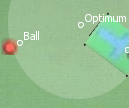
\includegraphics[width=0.13\textwidth] {optimumarea.png}
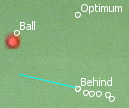
\includegraphics[width=0.13\textwidth] {behindprediction.png}
\end{center}
\caption{Threshold visualization and movement prediction}
\label{fig:orientation}
\end{figure}

\end{document}

